\subsection{Path following}\label{sec:prob2.2}
\begin{wrapfigure}{R}{0.4 \textwidth}
   \vspace{-30pt}
   \begin{center}
    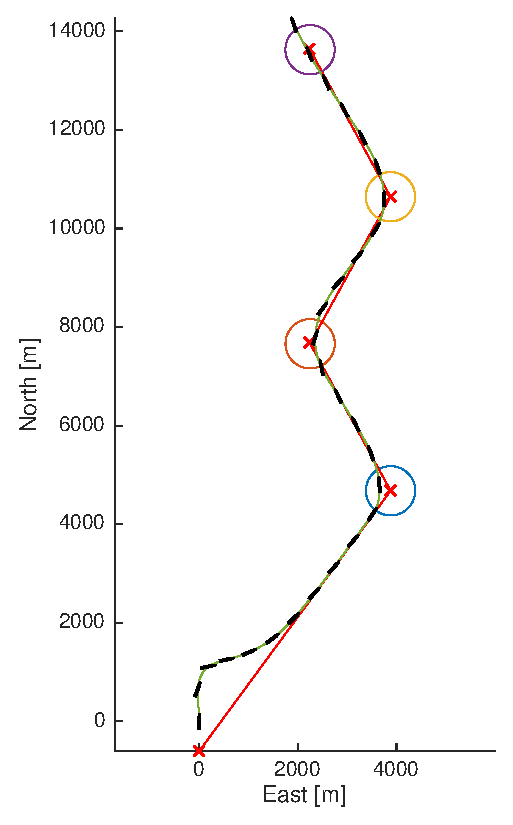
\includegraphics[width=0.6\textwidth]{task2.3/Task2_3-1}
    \caption{Path following}
   \end{center}
    \label{fig:2.3-path}
\end{wrapfigure}

We implemented a lookahead-based steering law, based on figure (10.10) in Fossen (2011). The desired course $\chi_d$ is made up of two parts, a path-angle $\chi_p$ and a cross-track error correction $\chi_r$. The cross-track error correction is essentially a PI-controller, normalized with an inverse tangent. The proportional gain is the inverse of the lookahead distance $\Delta_s$ which is a design parameter.
\begin{equation}
	K_p = \frac{1}{\Delta_s}
\end{equation}
The integral effect of the controller is quite complex, since we only want the integrator to compensate for small slow-changing disturbances like wind and current. To achieve this, we made an integral structure that takes into consideration the yaw rate of the ship $r$, the cross-track error $e$, a soft maximum integral effect and an anti-wind-up corrector and a regular gain on the end result. The total control law is listed in equation \ref{eq:PI-control-law}.
\begin{equation}
\begin{split}
	\chi_d &= \chi_p + \chi_r \\
	\chi_r &= atan(P - I) \\
	P &= K_p e \\
	I &= \int K_i e_i \\
	e_i &=	\begin{cases}
			0,								& \text{if}\ | r | > r_{lim} \text{ or }  | e | > e_{lim} \\
      			\frac{e}{k_1+k_2 \frac{| I |}{I_{max}}},		& \text{if}\ (I > I_{max} \text{ and } e>0) \text{ or }( I< -I_{max} \text{ and } e<0 )
      			\end{cases}
\end{split}
\label{eq:PI-control-law}
\end{equation}



\begin{figure}
   \centering
    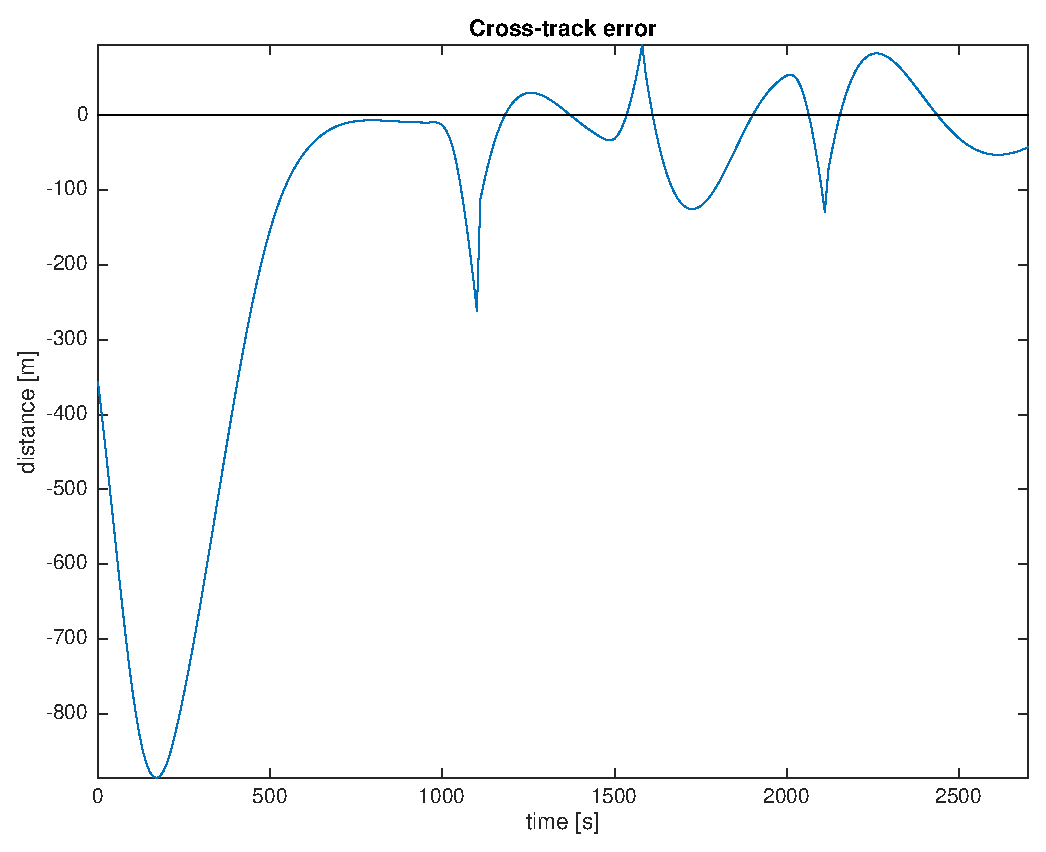
\includegraphics[width= \textwidth, height = 200pt]{task2.3/Task2_3-2}
    \caption{Cross-track error}
    \label{fig:2.3-error}
\end{figure}